\documentclass[10pt]{article}
\usepackage[margin=1in, paperwidth=8.5in, paperheight=11in]{geometry}
\usepackage{ifpdf,amsmath, amssymb, comment, color, graphicx, stmaryrd,setspace,enumitem,tikz, fancyhdr, wrapfig, textcomp, units, mathptmx, siunitx}

\usepackage{hyperref}
\hypersetup{
    colorlinks=true,
    urlcolor=blue,
}

\setlength{\headheight}{14.5pt}
\newcommand{\Q}{\mathbb{Q}}
\newcommand{\R}{\mathbb{R}}
\newcommand{\Z}{\mathbb{Z}}
\newcommand{\vu}{\mathbf{u}}
\newcommand{\vv}{\mathbf{v}}
\newcommand{\vw}{\mathbf{w}}
\newcommand{\vi}{\mathbf{i}}
\newcommand{\vj}{\mathbf{j}}
\newcommand{\vk}{\mathbf{k}}

% Solution text is in red. If you want the solutions to show, remove the \iffalse from the definition of the \red command.
\newenvironment{red}{\color{red}}{\ignorespacesafterend}
\newcommand{\blue}[1]{\textcolor{blue}{#1}}
\newcommand{\green}[1]{\textcolor{green}{#1}}
\renewcommand{\section}[1]{\begin{center} \textbf{#1} \\\end{center}}
%
\hyphenpenalty=5000
\setlength{\parindent}{0in}
%\oddsidemargin=-.25in
\allowdisplaybreaks
\pagestyle{fancy}
\renewcommand{\headrulewidth}{0pt}
\lhead{MATH 203}
\rhead{Spring 2020}
%\lfoot{\copyright\ CLEAR Calculus 2010}
\cfoot{}

\begin{document}
%


%\onehalfspacing
\allowdisplaybreaks
%##################################################################
\section{PS\#2: Multivariate functions - \red{Answer key} }

\begin{enumerate}[leftmargin=0pt]
    \item (ACM 9.1 Exercise 15) The Ideal Gas Law, $PV = RT$, relates the pressure ($P$, in pascals), temperature ($T$, in Kelvin), and volume ($V$, in cubic meters) of 1 mole of a gas ($R = \SI[per-mode=fraction]{8.314}{\J\per\mol\per\K}$ is the universal gas constant), and describes the behavior of gases that do not liquefy easily, such as oxygen and hydrogen. We can solve the ideal gas law for the volume and hence treat the volume as a function of the pressure and temperature:
    \[V(P, T) = \frac{8.314T}{P}.\]
    \begin{enumerate}
        \item Explain in detail what the trace of $V$ with $P = 1000$ tells us about a key relationship between two quantities.
        
        \begin{red}
        When $P = 1000$, $V(1000, T) = \frac{8.314}{1000} T$. That is, volume increases linearly with temperature, when pressure is held constant. (In fact, even better: volume is \textit{proportional} to temperature if pressure is held constant.)
        \end{red}
        \item Explain in detail what the trace of $V$ with $T = 5$ tells us.
        
        \begin{red}
        When $T = 5$, $V(P, 5) = \frac{41.57}{P}$. That is, volume is \textit{inversely} proportional to pressure, when temperature is held constant: if the pressure gets higher, the volume gets lower, and if the pressure gets lower, the volume gets higher.
        \end{red}
        \item Explain in detail what the level curve $V = 0.5$ tells us.
        
        \begin{red}
        If $V = 0.5$:
        \begin{align*}
            0.5 &= \frac{8.314 T}{P}\\
            P &= \frac{8.314}{0.5} T = 16.628 T
        \end{align*}
        This tells us that at constant volume, temperature is proportional to pressure (or, equivalently, pressure is proportional to temperature).
        \end{red}
        \item Use 2 or three additional traces in each direction to make a rough sketch of the surface over the domain of $V$ where $P$ and $T$ are each nonnegative. Write at least one sentence that describes the way the surface looks.
        
        \begin{red}
        Okay, so we've got linear level curves, linear $P$-traces, and $T$-traces that look like $1/P$. So $V$ increases linearly in the $T$ direction, and decreases asymptotically in the $P$ direction.
        
        Here's a graph of $z = 8.314 x/y$ in CalcPlot3D: \href{https://www.monroecc.edu/faculty/paulseeburger/calcnsf/CalcPlot3D/?type=z;z=8.314x/y;visible=true;umin=0;umax=400;vmin=1;vmax=100000;grid=30;format=normal;alpha=-1;constcol=rgb(255,0,0);view=0;contourcolor=red;fixdomain=false&type=window;hsrmode=3;nomidpts=true;anaglyph=-1;center=8.143342228569376,4.968016931136566,3.0007974140782387,1;focus=0,0,0,1;up=-0.2318433831714125,0.0028667885942549737,0.9727489024423465,1;transparent=false;alpha=140;twoviews=false;unlinkviews=false;axisextension=0.7;xaxislabel=x;yaxislabel=y;zaxislabel=z;edgeson=true;faceson=true;showbox=true;showaxes=true;showticks=true;perspective=true;centerxpercent=0.5;centerypercent=0.5;rotationsteps=30;autospin=true;xygrid=false;yzgrid=false;xzgrid=false;gridsonbox=true;gridplanes=false;gridcolor=rgb(128,128,128);xmin=0;xmax=400;ymin=1;ymax=100000;zmin=0;zmax=2;xscale=100;yscale=10000;zscale=1;zcmin=0;zcmax=2;zoom=0.000035;xscalefactor=400;yscalefactor=1;zscalefactor=50000}{Click me}\end{red}
        
        \begin{center}
        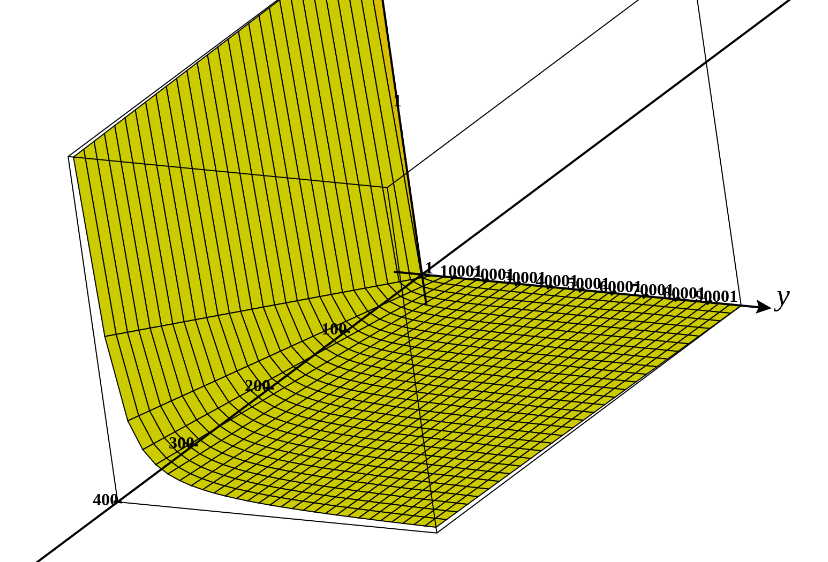
\includegraphics[width=0.5\textwidth]{203-keys/ps2-answer-key/ideal-gas.png}
        \end{center}
        \item Based on all your work above, write a couple of sentences that describe the effects that temperature and pressure have on volume.
        
        \red{Increasing temperature increases volume (proportionally). Increasing pressure decreases volume (in inverse proportion). If we hold volume constant, then increasing temperature increases pressure, and increasing pressure increases temperature.}
    \end{enumerate}
    \item (ACM 9.1 Exercise 16) When people buy a large ticket item like a car or a house, they often take out a loan to make the purchase. The loan is paid back in monthly installments until the entire amount of the loan, plus interest, is paid. The monthly payment that the borrower has to make depends on the amount $P$ of money borrowed (called the principal), the duration $t$ of the loan in years, and the interest rate $r$. For example, if we borrow \$18,000 to buy a car, the monthly payment $M$ that we need to make to pay off the loan is given by the formula \[M(r,t) = \frac{1500r}{1-\frac{1}{\left(1+\frac{r}{12}\right)^{12t}}}.\]
    \begin{enumerate}
        \item Find the monthly payments on this loan if the interest rate is 6\% and the duration of the loan is 5 years.
        
        \begin{red}
        \[M(0.06, 5) = \frac{1500\cdot 0.06}
        {1-\frac{1}{\left(1+\frac{0.06}{12}\right)^{12\cdot 5}}} = \$347.99.\]
        (Thanks, Wolfram$|$Alpha!)
        \end{red}
        \item Create a table of values that illustrates the trace of $M$ with $r$ fixed at 5\%. Use yearly values of $t$ from 2 to 6. Round payments to the nearest penny. Explain in detail in words what this trace tells us about $M$.
        
        \begin{red}
        \[
        \begin{array}{c|c|c|c|c|c}
            t          & 2        & 3        & 4        & 5        & 6        \\
            \hline
            M(0.05, t) & \$789.69 & \$539.48 & \$414.53 & \$339.68 & \$289.89
        \end{array}
        \]
        So this tells us that at a fixed interest rate, extending the loan duration decreases the monthly payments (in fact, by a decreasing amount).
        \end{red}
        \item Create a table of values that illustrates the trace of $M$ with $t$ fixed at 3 years. Use rates from 3\% to 11\% in increments of 2\%. Round payments to the nearest penny. Explain in detail what this trace tells us about $M$.
        
        \begin{red}
        \[
        \begin{array}{c|c|c|c|c|c}
            r       & 3\%      & 5\%      & 7\%      & 9\%      & 11\%     \\ \hline
            M(r, 3) & \$523.46 & \$539.48 & \$555.79 & \$572.40 & \$589.30
        \end{array}
        \]
        So this tells us that at a fixed loan duration, increasing the interest rate increases the monthly payment (in fact, by an amount that is sliiiiiiightly increasing).
        \end{red}
        \item Consider the combinations of interest rates and durations of loans that result in a monthly payment of \$200. Solve the equation $M(r, t) = 200$ for $t$ to write the duration of the loan in terms of the interest rate. Graph this level curve and explain as best you can the relationship between $t$ and $r$.
        
        \begin{red}
        Algebra time:
        \begin{align*}
            200 &= \frac{1500r}{1-\frac{1}{\left(1+\frac{r}{12}\right)^{12t}}}\\
            200\left[1-\left(1+\frac{r}{12}\right)^{-12t}\right] &= 1500r \\
            1-\left(1+\frac{r}{12}\right)^{-12t} &= 7.5 r \\
            1-7.5r &= \left(1+\frac{r}{12}\right)^{-12t}\\
            \ln(1-7.5r) &= -12t \cdot \ln\left(1+\frac{r}{12}\right) \\
            t &= \frac{\ln(1-7.5r)}{-12\ln\left(1+\frac{r}{12}\right)}
        \end{align*}
        Okay, so that's a perfectly fine function of $r$ that we now have for $t$. We can graph it:\\
        \begin{center}
            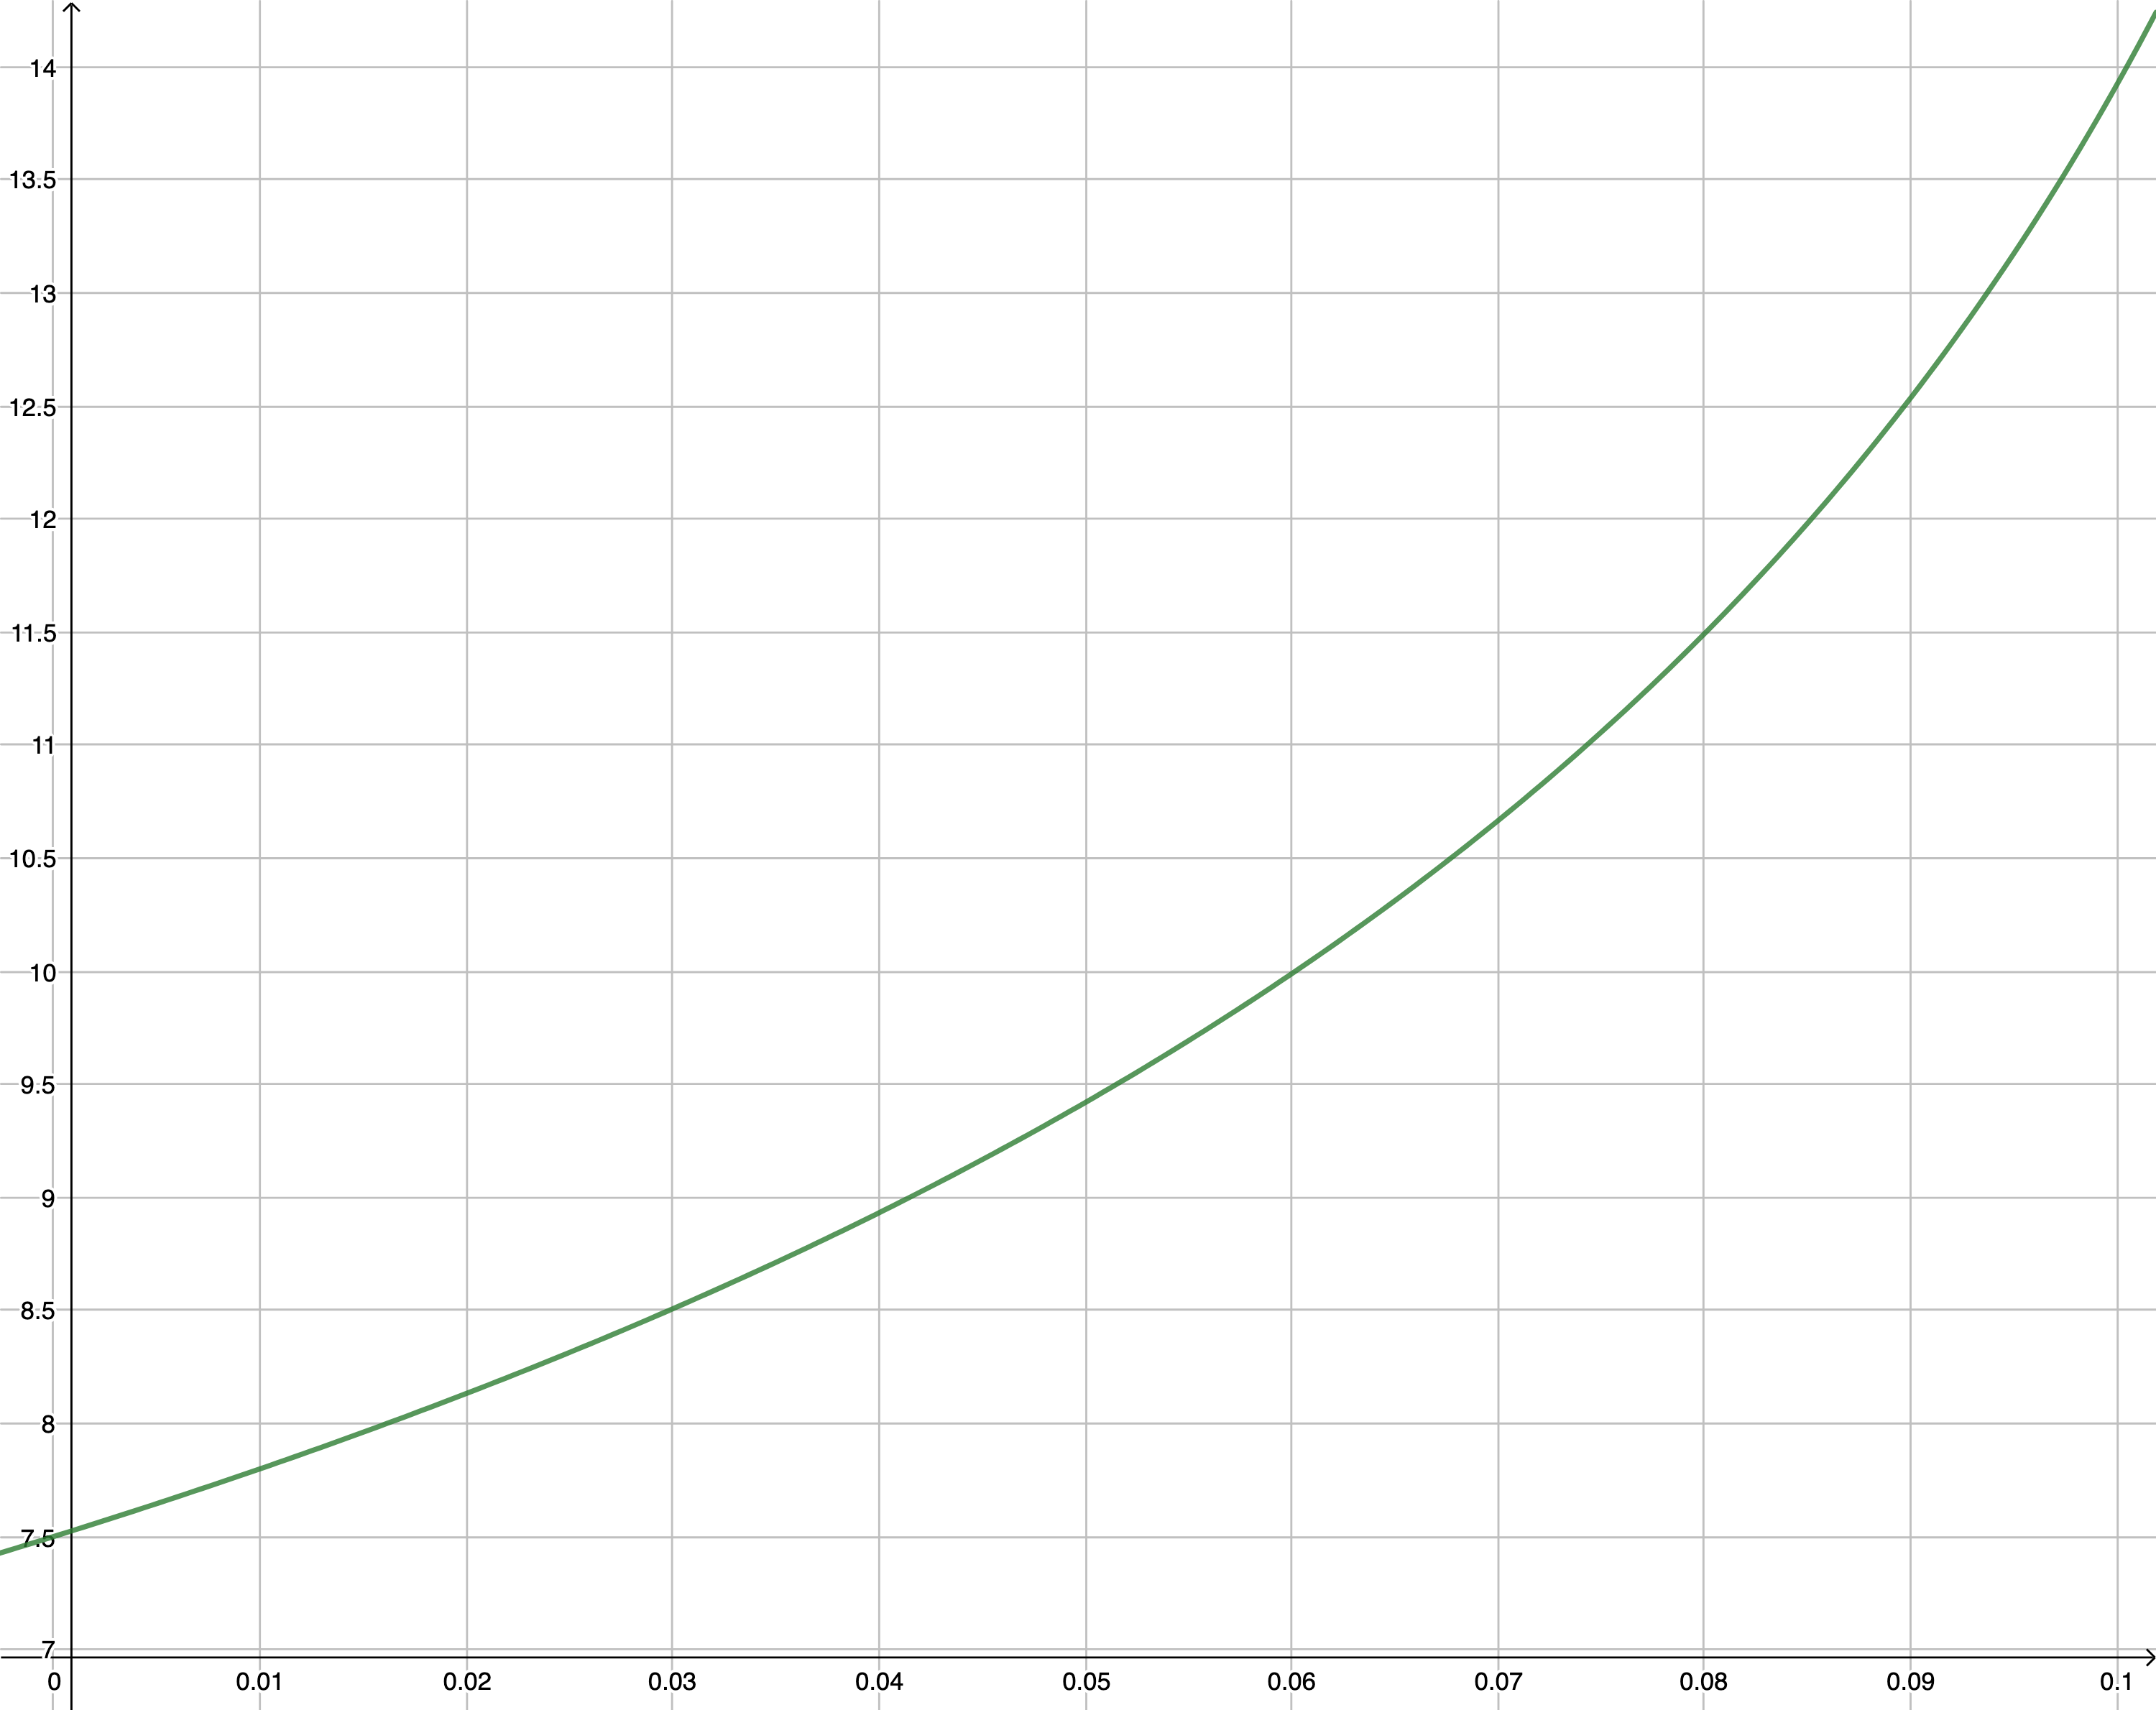
\includegraphics[scale=0.09]{geogebra-export.png}\\
        \end{center}
        (I used Geogebra to generate this graph, because Wolfram$|$Alpha insisted that the graph should be polar since it involved an $r$, and I couldn't figure out a good way to tell it that no, honestly, this is a rectangular plot, just with weird variable letters.)
        
        Some notes on the domain and range: reasonable values of $r$ are probably very small, because $r$ is our interest rate written as a proportion -- that is, an interest rate of $5\%$ is written as $r = 0.05$. $t$ is the number of years, so we can expect it to be probably around 10 or something.
        
        So, if we want to have a fixed monthly payment of \$200, then increasing the duration will force us to increase the interest rate, and increasing the interest rate will force us to increase the duration.
        
        (In other words that are more practical: if we're offered a lower interest rate and we want to keep our payments the same, then we can pay off the loan in a shorter duration.)
        \end{red}
    \end{enumerate}
\end{enumerate}

\end{document}